\section{Contextualização}
\par
Atualmente a sociedade vive rodeada de tecnologias indispensáveis e de ambientes que se intitulam Smart, mas nem sempre foi assim.\par
Desde cedo, mesmo antes de existir tecnologia, o homem tendeu a procurar e encontrar coisas que melhorassem a sua vida e bem-estar pessoal e da sociedade, mas para chegar a humanidade está hoje é necessário recuar na história algum tempo para marcos importantes da tecnologia.\par
Um dos marcos muito importantes para o desenvolvimento dos sistemas embebidos e de sistemas de monotorização foi a invenção dos processadores. Com o surgimento dos processadores começaram a surgir os primeiros sistemas embebidos e sistemas de monotorização. Com o passar dos anos até aos dias de hoje a tecnologia tem vindo a evoluir e por consequência os sistemas também se adaptaram para os padrões de atualmente.\par
Uma das partes mais importantes num sistema embebido é a sua interface disponível para o utilizador, as principais e mais usadas nos dias de hoje são a linha de comandos e a WEB, comuns para configurações á distância e as interfaces dos próprios equipamentos como os ecrãs com software proprietário.

\section{A Empresa}
\par
A empresa CapTemp, Lda localizada em Pombal, Leiria é uma empresa, focada em desenvolvimento de soluções de monotorização, controlo, supervisão e de soluções á medida consoante os requisitos do cliente. Para criar um sistema de monotorização é necessário o sistema possuir sensores, atuadores, coletores de dados e software para analisar os dados provenientes dos sensores de modo a possuir capacidade de atuar com base nesses valores. A Captemp é responsável pelo desenvolvimento de todos estes componentes passando pelos sensores até ao software responsável por analisar e armazenar os dados.\par
Uma das subáreas da empresa é a disponibilização de um Registador de temperatura e respetivo Software certificado para Meteorologia Legal.
Faz parte deste conjunto o Software “CapTemp SQL” representado na figura \ref{figcaptempsql} responsável por guardar os dados provenientes dos sensores ligados ao registador.\par
\begin{figure}[ht]
  \centering
  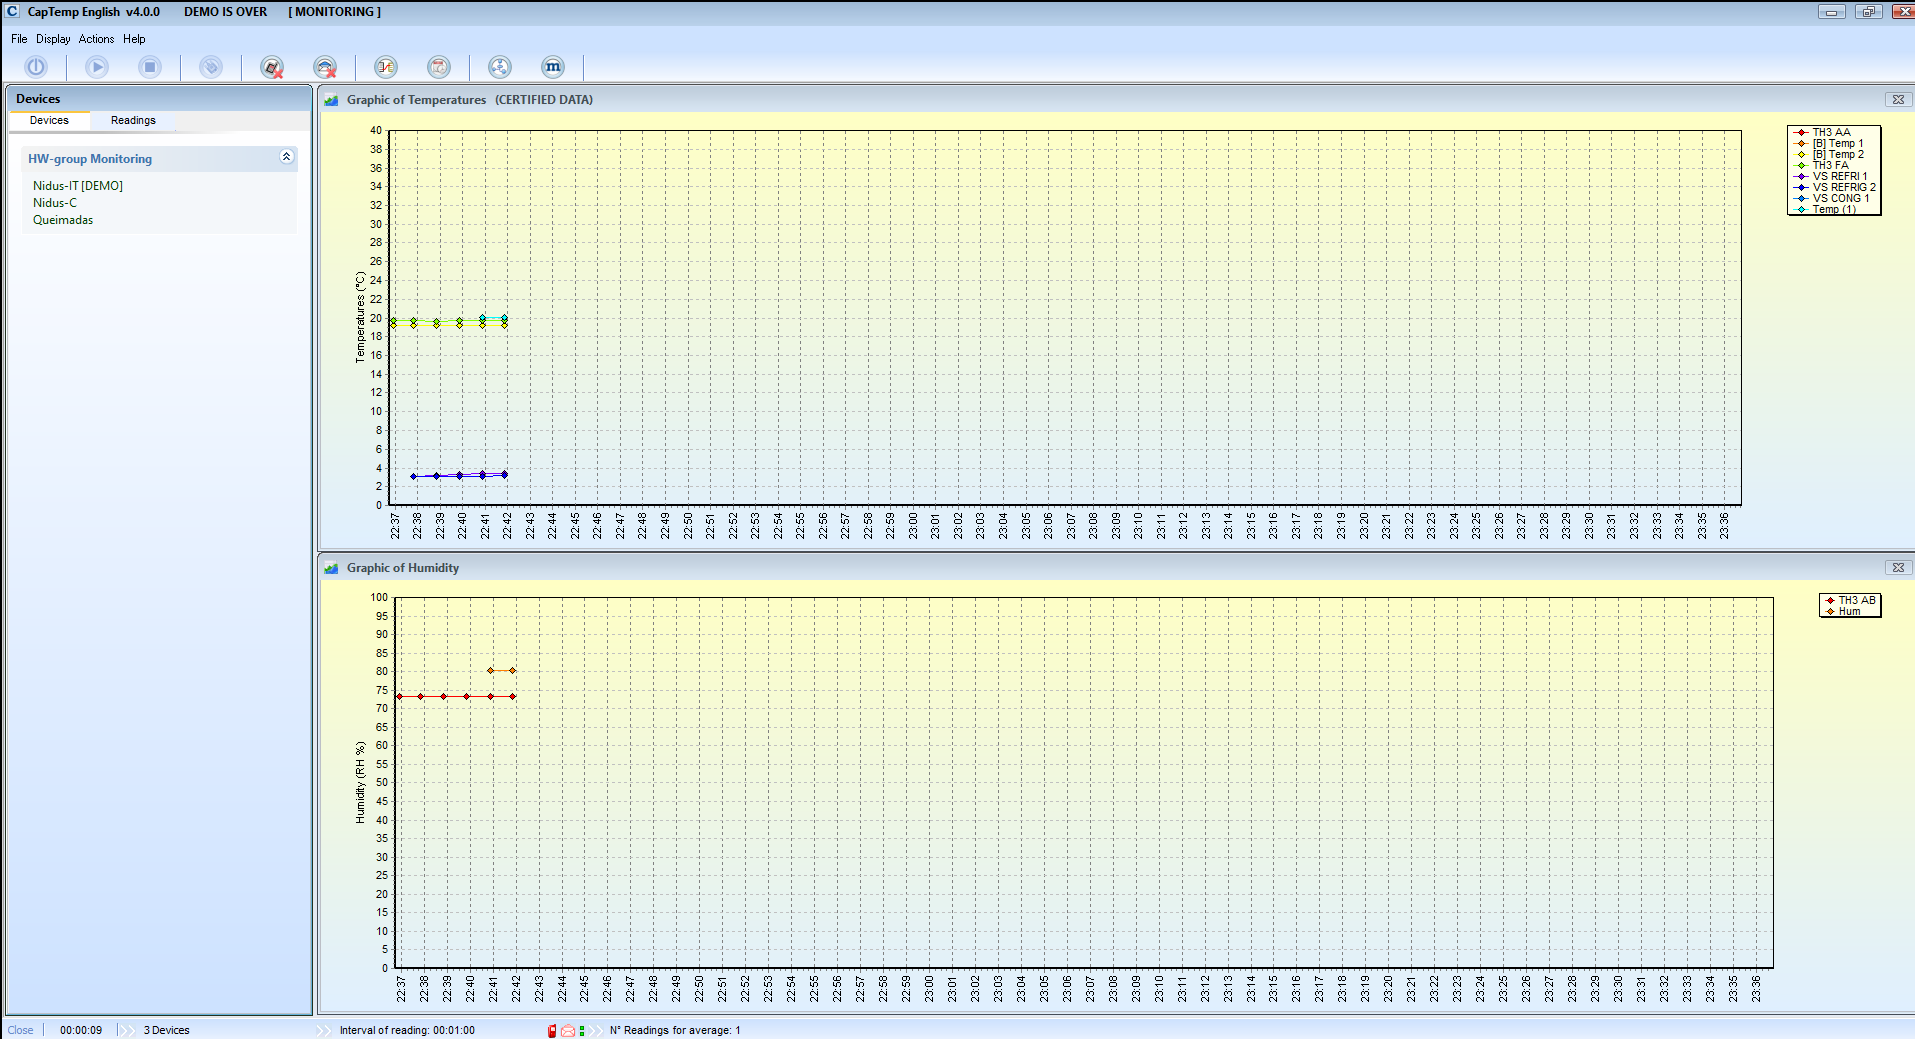
\includegraphics[width=1.00\textwidth]{images/captemp.png}
  \caption{CapTemp SQL}\label{figcaptempsql}
\end{figure}
O registador desenvolvido pela Captemp, representado na figura \ref{fignidusCl} denomina-se por Nidus-C, um registador que suporta até 32 sensores.\par

\begin{figure}[ht]
  \centering
  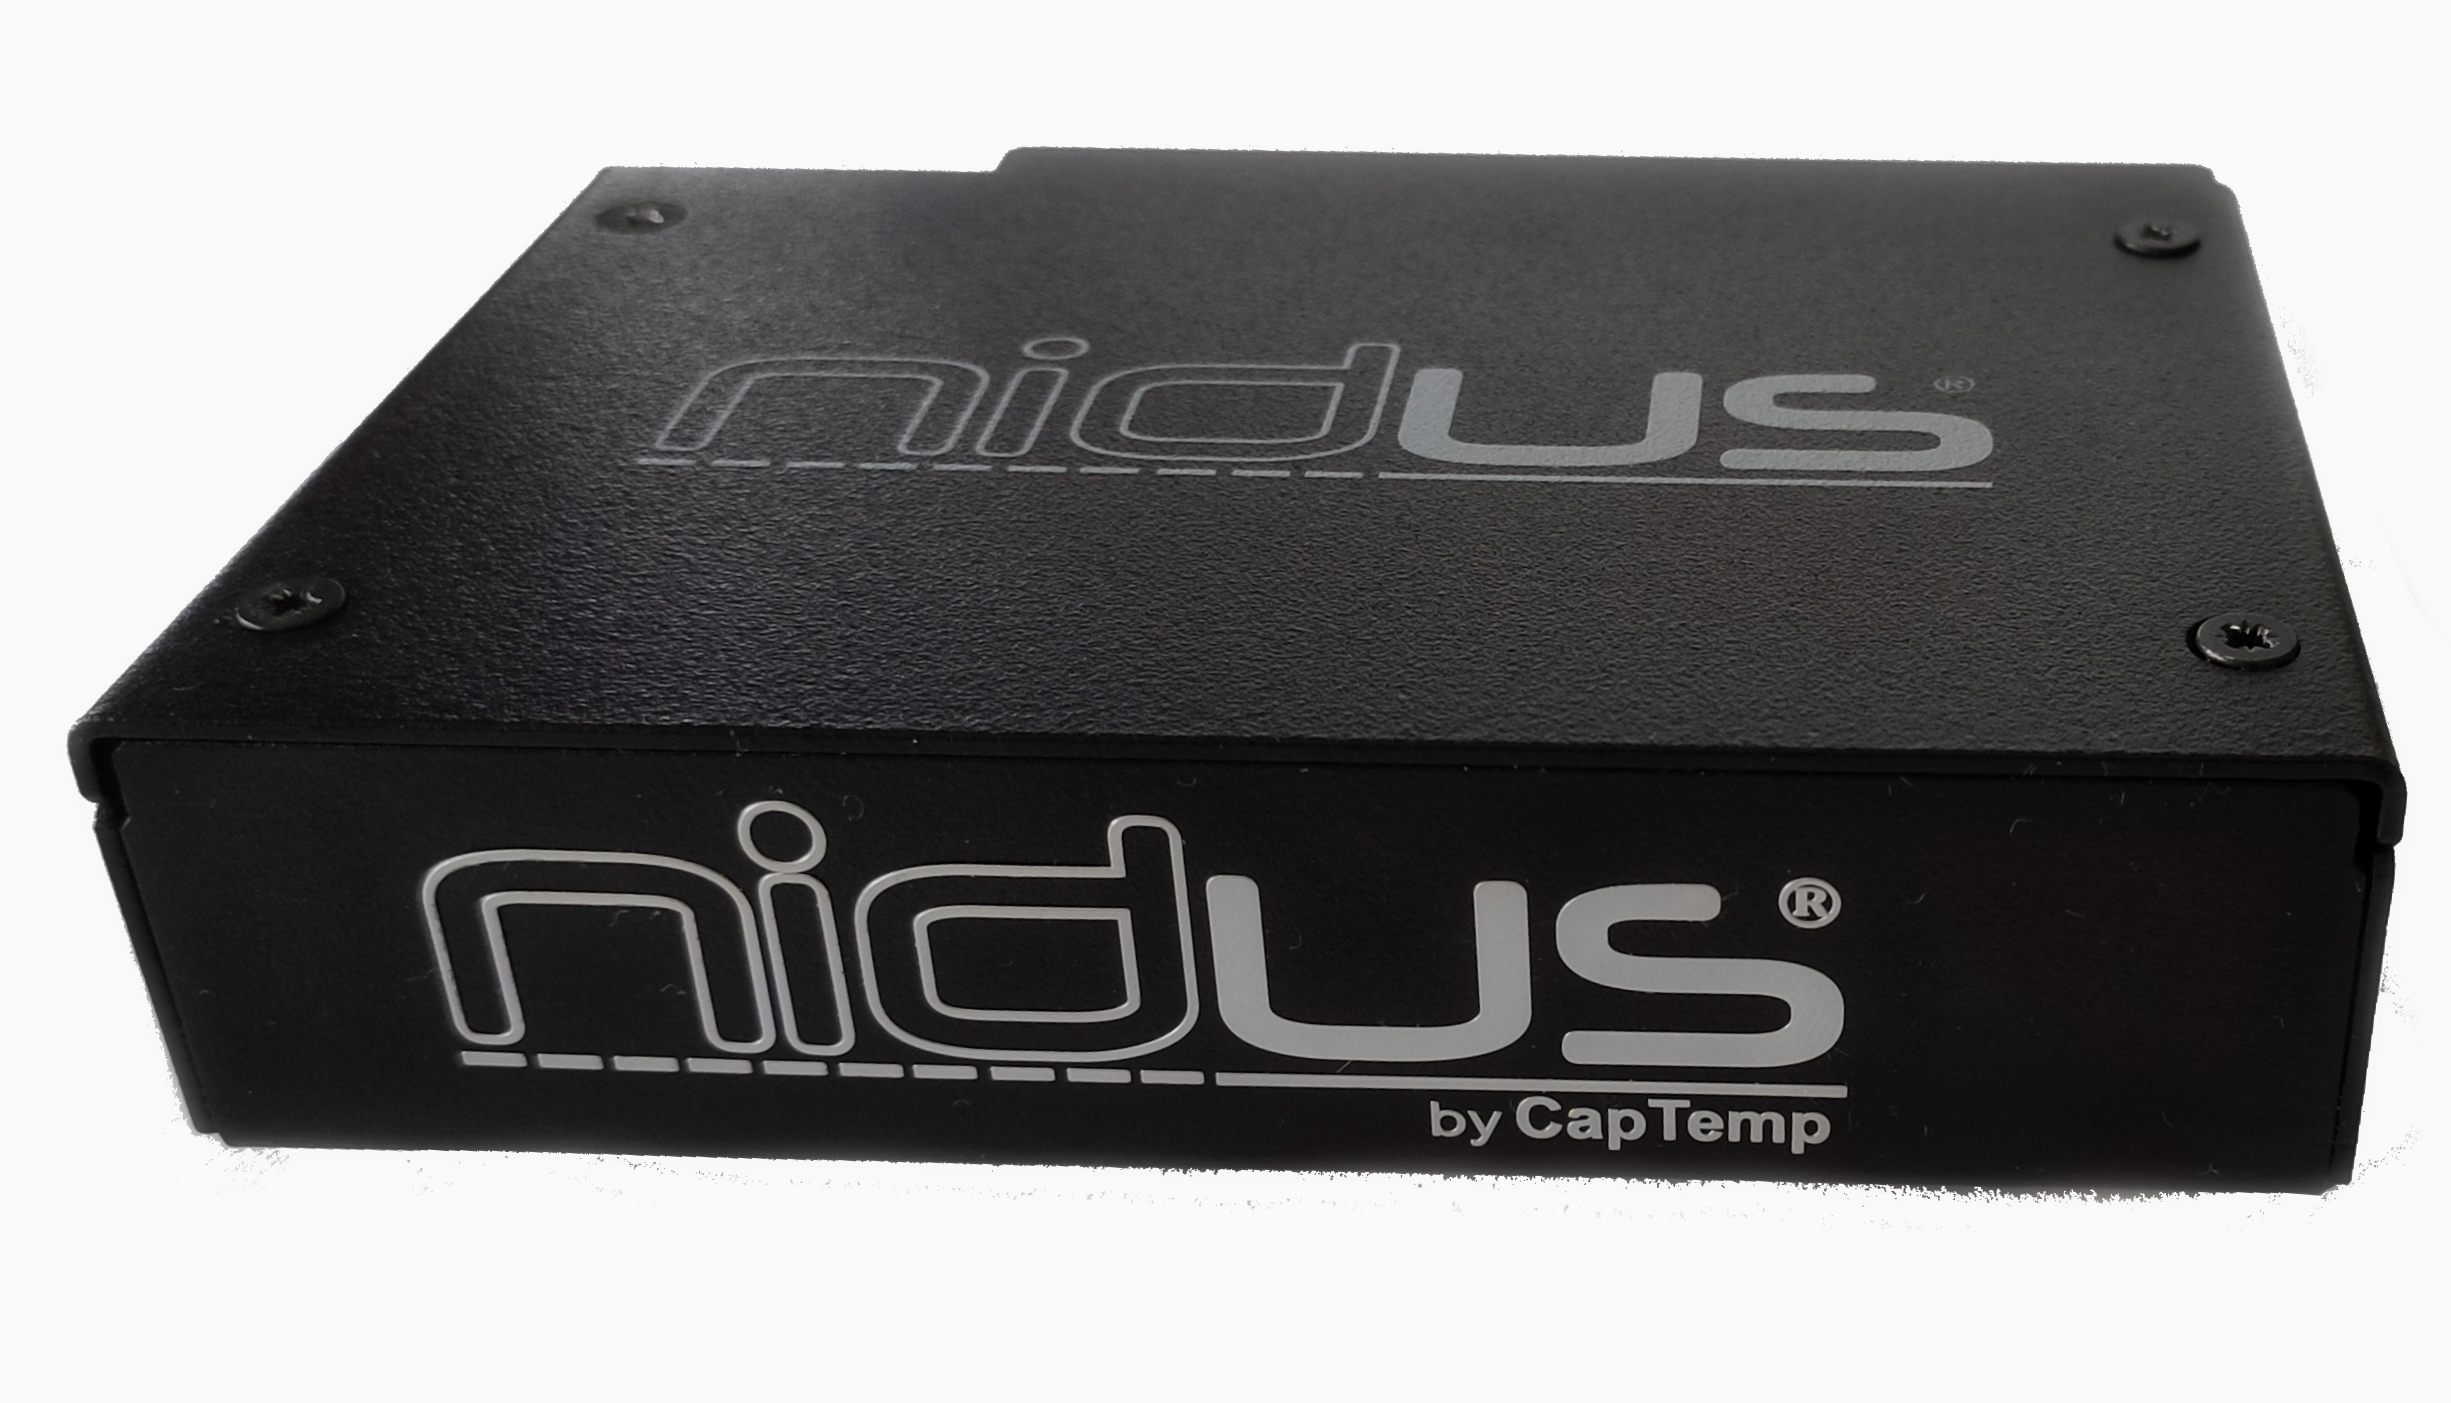
\includegraphics[width=0.45\textwidth]{images/nidus.jpg}
  \caption{Coletor de Dados Nidus-C}\label{fignidusCl}
\end{figure}

Com a necessidade de mais funcionalidades, a Captemp criou várias variantes da Nidus-C, representadas na Figura \ref{fignidusall} para aplicar em outras áreas para além da Meteorologia Legal. Das quais surgiram a Nidus-C+, similar á Nidus-C acrescentando a possibilidade de adicionar sensores Wireless. A Nidus-IT e Nidus-IT+ duas versões com as funcionalidades da Nidus-C e Nidus-C+ respetivamente, acrescentando Inputs e Outputs ao sistema de monotorização. Para soluções exclusivamente Wireless nasce a Nidus-W suportando apenas sensores Wireless. Por último é desenvolvido a Nidus-R, baseada na Nidus-IT especialmente desenhada a pensar em ambientes IT com suporte para montagem em bastidores.
\par
\begin{figure}[ht]
  \centering
  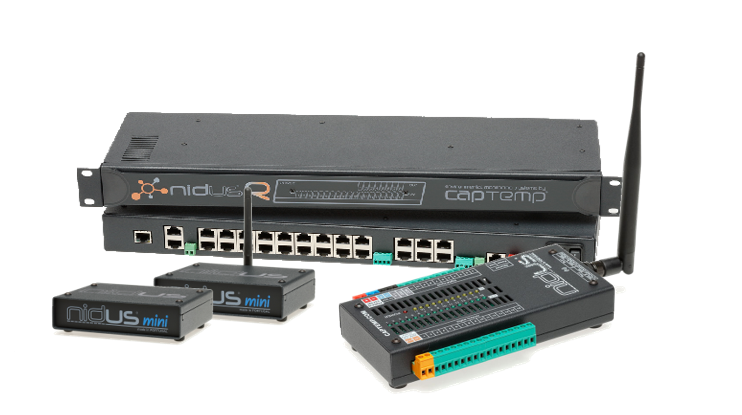
\includegraphics[width=0.65\textwidth]{images/nidusall.png}
  \caption{Universo Nidus}\label{fignidusall}
\end{figure}

No setor dos sensores foi desenvolvido o TH3 um conversor RS485 permitindo às diversas Nidus, ligar por RS485 a sensores 1Wire além dos dois inputs possuídos no TH3. Nos sensores wireless, foi desenvolvido o Airo á semelhança do TH3 possui dois inputs, um ecrã e possibilita a ligação de sensores. Permite ainda a leitura de todos os Airo adicionados á Nidus ao mesmo tempo, tecnologia desenvolvida pela Captemp denominada por Captemp AST \cite{Captemp_AST}. Ambos os sensores estão representados na Figura \ref{figairoth3} 
\begin{figure}[ht]
  \centering
  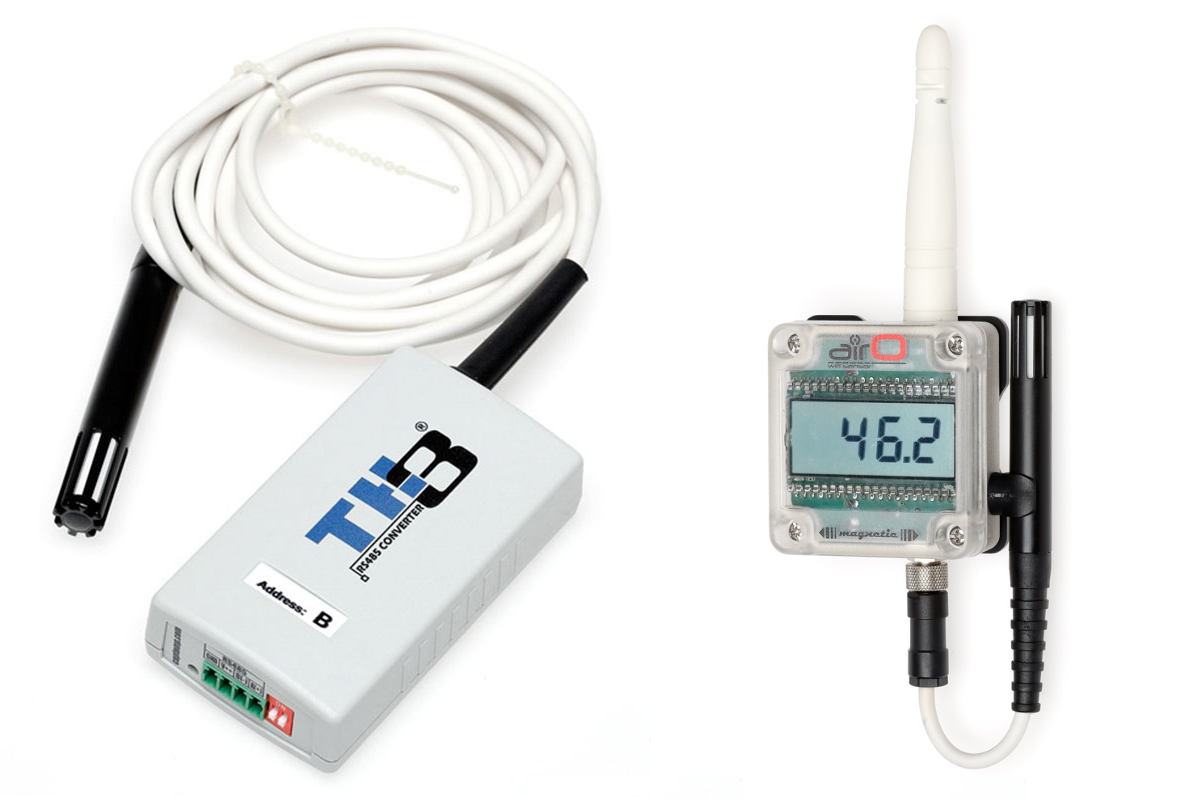
\includegraphics[width=0.45\textwidth]{images/th3airo.png}
  \caption{ TH3 e Airo}\label{figairoth3}
\end{figure}
\par
Em desenvolvimento encontram-se sensores com recurso a tecnologias NB-Iot, Beacon's BLE e Lora.
\par
A Captemp desenvolve igualmente um portal Cloud denominado Senslive(Figura \ref{figsenslive}) que possibilita a centralização dos sistemas de monotorização numa plataforma Cloud.

\begin{figure}[ht]
  \centering
  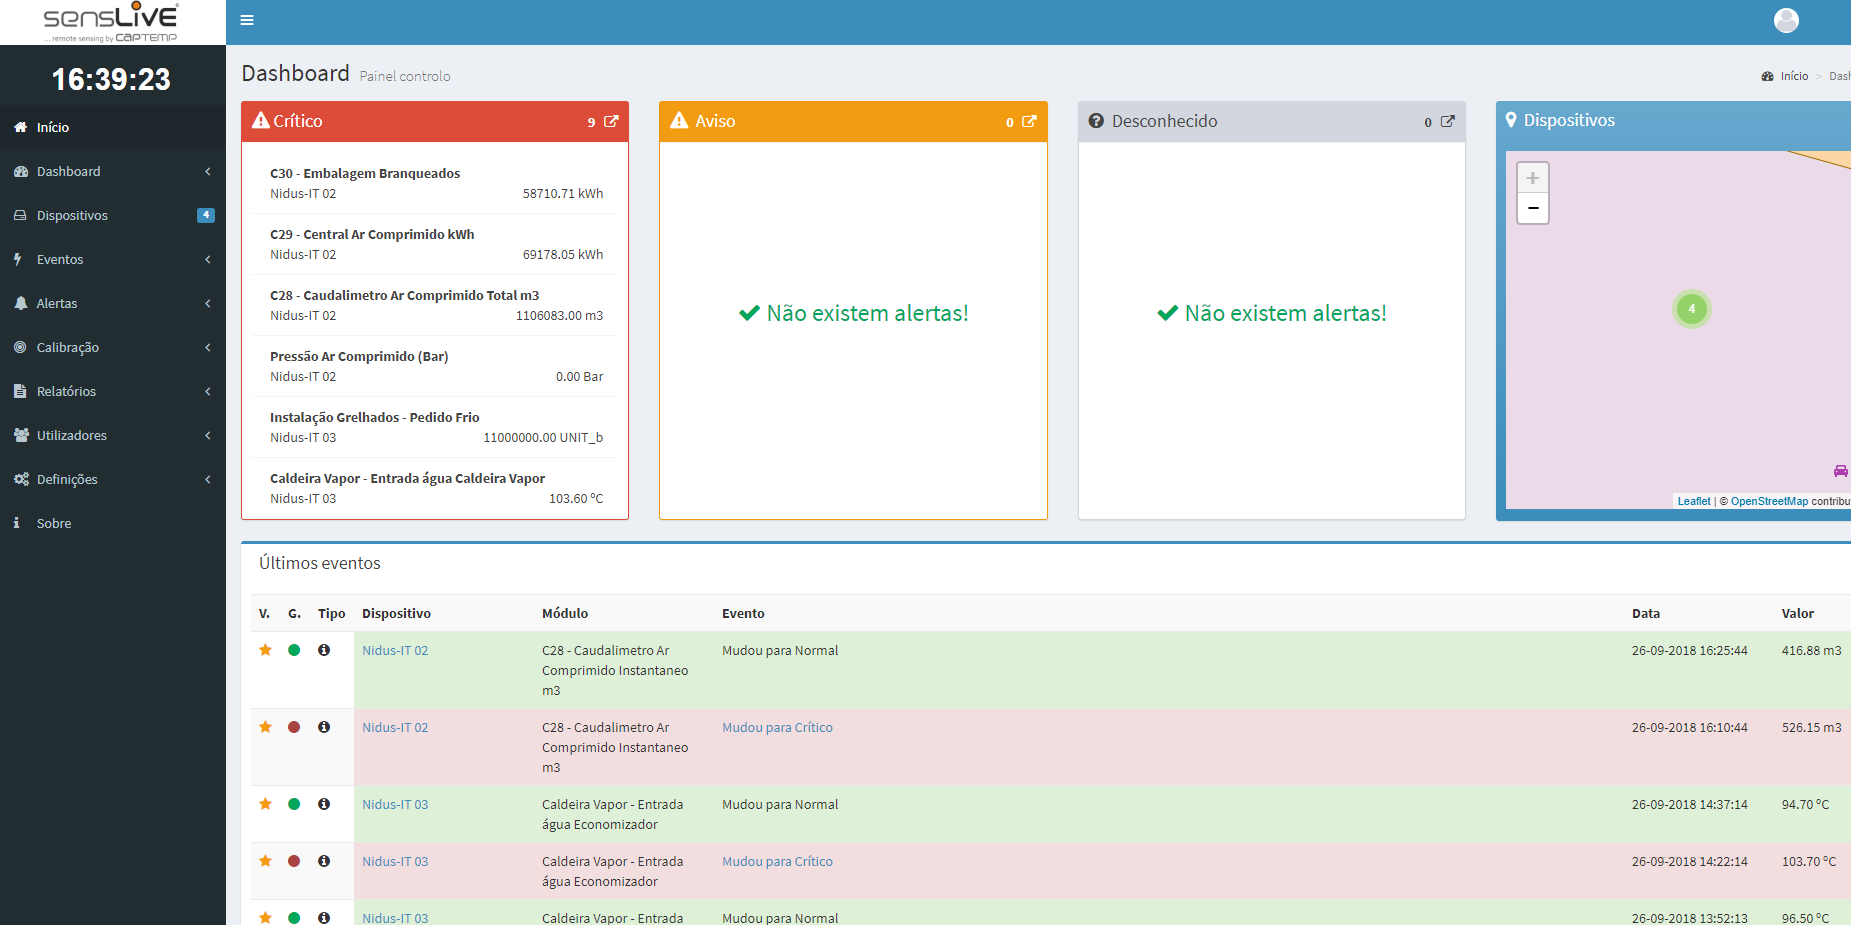
\includegraphics[width=0.95\textwidth]{images/mwsnap0791.png}
  \caption{ Portal Senslive}\label{figsenslive}
\end{figure}



\section{Motivação e Objetivos}
\par
O estágio é uma forma do estudante colocar numa situação de contexto profissional os conceitos adquiridos em contexto académico. A realização de um estágio é também uma mais valia pois possibilita o adquirir de experiência profissional que não é possível obter em contexto escolar.
\par
Ao longo do estágio, serão aplicados vários conhecimentos adquiridos durante o percurso académico de modo a melhorar a interface para o utilizador, técnicas de otimização de código, compressão de ficheiros, manipulação de imagens de modo a ocupar o mínimo de espaço permitindo futuros desenvolvimento e melhorias, dando continuidade ao suporte do projeto Nidus, igualmente serão criados dois novos projetos de desenvolvimento de novos equipamentos que tiram partido de novas tecnologias como o NB-Iot e Beacon’s BLE.
\subsection{Nidus}
\par
O projeto "Nidus" tem como objetivo dar suporte ao Front-end das Nidus já existentes para correções de bugs encontrados em versões anteriores, otimização de código, de modo a ocupar o mínimo espaço, possibilitando deixar memória livre para desenvolvimentos futuros, desenvolver versões customizadas com layouts a pedido do cliente com funcionalidades especificas, ou simplesmente melhorar a página seguindo a tendência de equipamentos concorrentes.
\subsection{NB-Iot}
Com o surgimento da nova tecnologia NB-Iot surgiu a necessidade de serem criados equipamentos que tirem partido dessa tecnologia e as suas vantagens. Para tal durante o estágio será desenvolvido um dos equipamentos que tira partido da tecnologia. Este projeto tem como por objetivo criar uma versão de raiz, simplificada e mais barata de um outro equipamento de NB-Iot em desenvolvimento pela Captemp, através do módulo Xbee da DIGI e da sua programação em Micropython. Durante o projeto será necessário garantir a correta gestão de memória, gestão de Logs internos, comunicação com os sensores físicos, comunicação bidirecional e encriptação com o portal Senslive.
\subsection{Kea Tracker}
O "Kea Tracker" é um projeto de Beacon’s BLE que comunicam com o smartphone, onde é possível definir alertas locais no smartphone e envio dos dados obtidos dos sensores das beacon’s e envio para a plataforma Senslive.
Tal como o projeto anterior será necessário além de criar uma aplicação para smartphone, criar Firmware específico para as beacon’s que na ausência de comunicação com o smartphone devem armazenar em Log as leituras dos sensores e quando este está ao alcance descarregar para o smartphone.

\section{Os Problemas}
A página WEB da nidus desde a sua criação já sofreu muitas alterações para seguir os padrões e tendências da concorrência e portanto está em constante atualização. Hoje em dia com a mundialização quase todas as pessoas sabem inglês e usam sistemas em inglês, mas existem algumas pessoas que ou não sabem ou preferem usar a lingua nativa preferem ter o sistema na sua lingua, para tal a captemp pretende desenvolver uma página WEB com um sistema de tradução que seja possivel alojar na memória do equipamento para o utilizador escolher a linguagem a usar e assim cativar mais clientes a usar os equipamentos Captemp e expandir a Captemp para outros países. Com o acrescimo do sistema surge o problema de uma quantidade maior de código alojado na memória, irá ser revisto otimizações que se possam fazer no código já existente, irá ser estudado o melhor metodo de compressão da página mantendo o GZIP utilizado atualmente ou migrar para outro mais recente como o Brotli e compressão de imagens migrando as imagens existentes para imagens SVG, possibilitando outras soluções para a página com sistemas mais interativos e ocupando o menor espaço disponivel. Além dos problemas referidos anteriormente poderão surgir novas funcionalidades a implementar, a pedido do cliente, como por exemplo páginas com layout especificos ou novos sensores, ou a simples correção de possiveis Bugs encontrados nas versões em produção
\par
Outro problema a resolver detetado pelo feed-back recebido dos clientes é a complexidade para a criação de eventos, ações e reações, que controlam o Sistema Nidus. Para isso a Captemp pretende reformular a extrutura de gestão de eventos para um sistema mais visual  e atual similar ao Scratch, um software utilizado para ensinar a crianças as bases da programação e elas mesmos criarem alguns programas sem saber nenhuma linguagem de programção. Na figura \ref{scratch} é apresentado um exemplo de programação usando a ferramenta Scratch, onde o utilzador com um sistema de blocos pode criar condiçoes e eventos a despoltar consoante algumas condições.
\begin{figure}[ht]
  \centering
  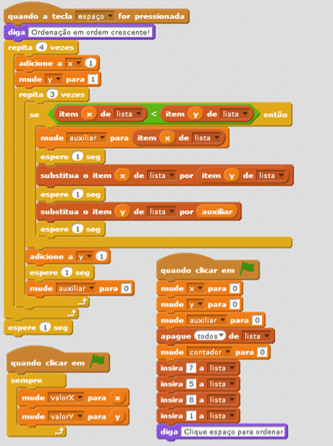
\includegraphics[width=0.55\textwidth]{images/scratch.png}
  \caption{ Programação com a ferramenta Scratch}\label{scratch}
\end{figure}

Outros problemas existentes,a resolver durante o estágio, são a criação de sistemas low-cost para o cliente que não necessita de tantas funcionalidades com a introdução da alternativa para NB-Iot com recurso ao módulo Xbee da Digi, e a substituição de produtos antigos deixados de ser comercializados pela Captemp, os data-logger(Figura \ref{ds1921}) compativeis com o Software Captemp SQL e sua substituição por similares com as mesmas fuções mas com os padrões e tecnologias dos dias de hoje e com suporte para o novo Portal da Captemp o Senslive.
\begin{figure}[htb]
  \centering
  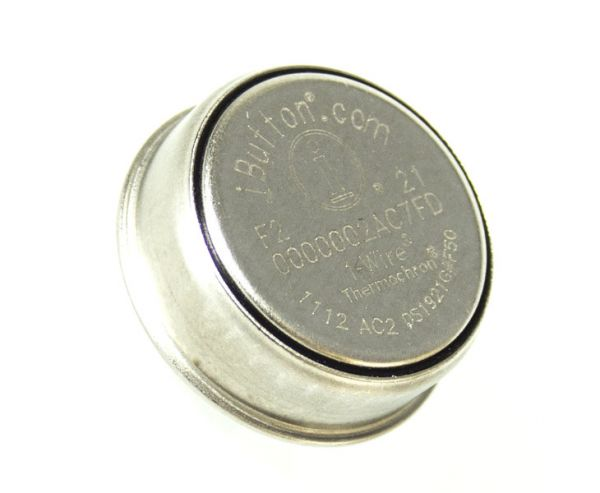
\includegraphics[width=0.25\textwidth]{images/ds1921.jpg}
  \caption{Data Logger iButton}\label{ds1921}
\end{figure}
\par
Em resumo os problemas a solucionar durante o estágio podem ser encontrados na seguinte enumeração:
\begin{itemize}
\item Melhorar a compressão da página WEB da Nidus;
\item Melhorar a compressão das imagens presentes na página WEB da Nidus;
\item Correção de Bugs da página Web da Nidus;
\item Melhoração do processo de criação de eventos;
\item Criação de uma página com sistema de tradução automático;
\item Versões costumizadas da página WEB a pedido do cliente;
\item Seguir as tendências da concorrencia;
\item Criação de soluções/equipamentos de baixo custo;
\item Substituição de produtos descontinuados;
\end{itemize}

\section{Organização do relatório}

{\color{red} \rule{\linewidth}{0.5mm} } 
A realizar no Fim da Estrutura completa\par
{\color{red} \rule{\linewidth}{0.5mm} } 
